\graphicspath{{chapters/06/images/}}
\chapter{Hybrid simulation approaches}

\section{Introduction}
Hybrid simulation approaches refer to a class of methods that combines the advantages of complementary simulation approaches: the system is partitioned into subsystems that are simulated with different methods.
When exact stochastic simulation is not a realistic option approximate strategies have to be considered together with their accuracy, so they often require the fulfilment of specific conditions.
The state space associated with biochemical reaction networks can be partitioned into regions depending on the nature of the system, according to the number of molecules and the frequency of reaction events.
This helps evaluate which approximations are reasonable.
The essential elements are the abundance of the species and the frequency of reaction.
Threshold variables demarcate the different partitions and they are model dependents as seen in figure \ref{fig:regions}:

\begin{multicols}{2}
  \begin{itemize}
    \item $t_1$ indicates whether a reaction is considered fast.
    \item $t_2$ indicates whether a population is abundant or not.
    \item $t_3$ and $t_4$ the border between stochastic variation and deterministic behaviour.
  \end{itemize}
\end{multicols}

\begin{figure}[H]
  \centering
  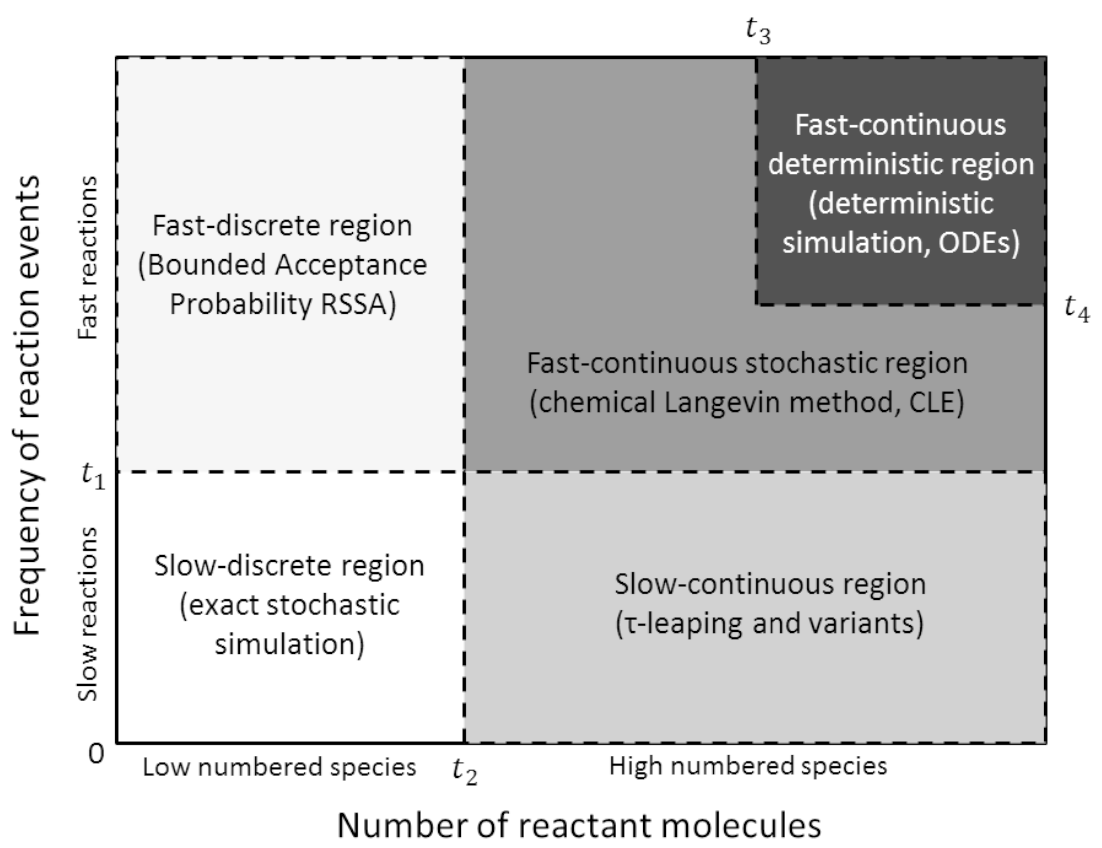
\includegraphics[width=0.5\textwidth]{regions.png}
  \caption{Partitions of the state space}
  \label{fig:regions}
\end{figure}

  \subsection{Slow-discrete region}
  The system is in a slow-discrete region when the reaction are slow and low numbered species are present.
  The species must be represented with an integer and discrete changes are allowed.
  Moreover the reaction events are rare and correspond to significant changes in the system.
  This region should be treated with the highest accuracy method available.

  \subsection{Fast-discrete region}
  The system is in the fast-discrete region whenever molecular populations are small and the reactions happen frequently enough that exact simulation could be intractable.
  This region can be treated with stochastic approximate algorithms developed to work with large reaction propensities and small populations like BA-RSSA.

  \subsection{Slow-continuous region}
  The system is in the slow-continuous region whenever molecular population are large and reaction are slow.
  The molecular populations can be assumed continuous and each reaction occurrence does not change significantly its species concentration.
  The simulation of many reaction occurrences can be skipped without affecting the accuracy.
  This region can be treated by the $\tau$-leaping algorithm.

  \subsection{Fast continuous stochastic and deterministic region}
  The system starts in the fast continuous stochastic and goes into the deterministic whenever it has fast reactions and high number species.
  In the first case the CLE can be considered for the simulation, while in the second deterministic simulations can be used.

  \subsection{Dimensionality explosion}
  The system is two dimensional only when it has one species and one reaction.
  When these two sets increase the criteria above can be applied only when all of them belong to the same region.
  This is a very strict condition that must be preserved along all of the simulation process.
  Hybrid simulation approaches try to solve this problem by dividing the system into parts that fit with the regions described which are then simulated by ad hoc simulation methods to provide the best compromise between accuracy and runtime.





\section{Reaction-Based System Partitioning}
In order to divide reactions into group we can set up a threshold, which could be computed over the product of the propensity of the state and the simulation step.
If the product is higher or lower than the threshold, we can identify the reaction as rare or probable.
Example of partitioning algorithm: \emph{two class reaction-based partitioning}.
Divide reactions in slow and fast through an iterative loop.
In general, we can increase the complexity of such approach as much as we want.
Example: \emph{four class reaction based partitioning}, we can bridge more simulation strategies.
In Algorithm 45 the four class partitioning is applied; at the very beginning we impose a time step e.g.~with tau leaping, compute the partitioning ending up with 4 sets (very slow, slow, medium and fast).
For any of the reactions we will apply different strategies, for instance in the case of the very slow we require exact stochastic simulation.
For sure the simulation will be more accurate, but we cannot claim that the simulation is exact, since we are only working on a set of reactions, not on the full system.
If we wish to have an exact algorithm, we should consider the problem of \textbf{time varying reaction propensity}.
If we want to be able to appropriately generate time, we should move considering the integral of the propensity over the time and the random number.
We can consider the zero crossing of an equation as following (the log of the random number is a negative quantity):

$$\int_t^{t+\tau}a_0^s (X(t')) dt' = - \ln(r)$$
\noindent
Instead of deciding $\tau$ at the beginning, the time will be computed along the approximation; when the quantity will be equal to zero, the approximation will stop and restart.
We can consider this as a sort of traffic light: an event is generated, green light, we can move one.
The real issue is that even if we have an equation to find the right time, being able to compute this requirement exactly with a computational strategy is a problem.
The approach to zero will be affected by a variety of steps, e.g.~the computer has a certain threshold for the zero.
In addition computing the integral is computationally challenging.

\begin{enumerate}
  \def\labelenumi{\arabic{enumi}.}
  \item non trivial complexity, integrals tend to be approximated by computers
  \item the zero crossing is affected by approximation error
\end{enumerate}
\noindent
If we use deterministic simulation for simulating fast reactions, we can add another equation to understand when it is the time to stop during the simulation.
We start from the logarithm of the random number and proceed with numerical integration.

$$\frac{dRES}{t}= a_0^x,RES(0)= \ln(r)$$

Synchronization has a price: the more complex, the higher impact we will have on the right time.
Can we do something better? We can apply an extension of RSSA to obtain better results.

\section{HRSSA}
This algorithm claims to be exact and was developed by Marchetti.
In RSSA we have a side effect: $\tau$ is computed over an \emph{upper bound}, therefore we no longer need to reason in terms of propensity varying in time.
By taking this perspective, we totally avoid slow events, just focus on upper bound.
We have two main issues in this strategy:

\begin{enumerate}
  \def\labelenumi{\arabic{enumi}.}
  \item by considering an upper bound we will generate more events
  \item the bounds should be satisfied, therefore along the simulations we will need to check the consistency over the fluctuation interval of the state
\end{enumerate}
\noindent
We have no need of computing the integral, we work with fluctuation intervals and link the generation of $\tau$ over this quantity, with the only difference that we only consider the upper bound and not the current value.
\\
\\
\noindent
Pseudocode (Figure \ref{fig:HRSSA}): we start from a while loop, we compute the fluctuation interval, the bounds of the propensity (same as RSSA) and move forward with $\tau$ computation.
\begin{figure}
  \centering
  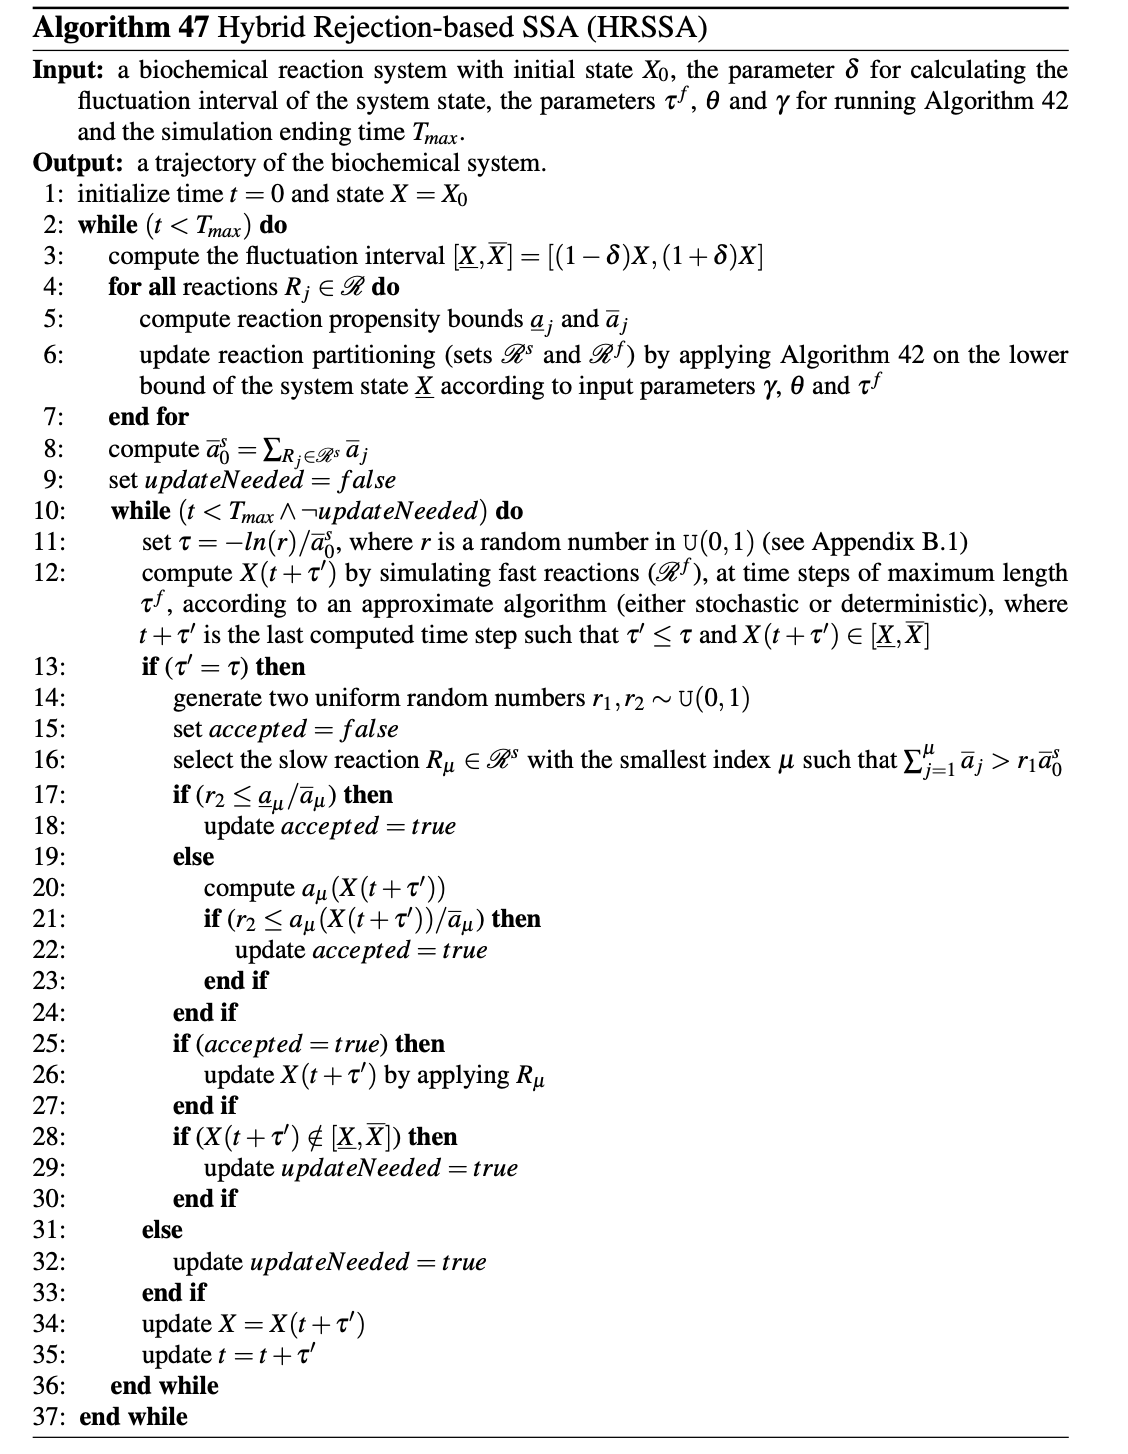
\includegraphics[width=0.5\textwidth]{HRSSA.png}
  \caption{HRSSA algorithm}
  \label{fig:HRSSA}
\end{figure}
When we reach $\tau$ we decide to apply or not the reaction through random number generation.
The main issue is how to compute the reaction partitioning, in this case the algorithm divide into slow and fast.
Since we are working with bounds, we substitute the real propensity with the lower bound for performing the partitioning.
Given that the partitioning is computed on the bound, it is just necessary to compute it again for each interval → speed up.
When the system is very complex, it is often not possible to apply this algorithm.

\subsubsection{HSimulator}
Simulator prototype (Java) developed by Marchetti to try HRSSA.
We simply provide the set of reactions in arrow notation, same specification as MATLAB.
The simulations provided are DM, RSSA, Euler, RK45 and HRSSA.
We have the possibility to define simulation length and time sampling i.e.~sampling over which the time series is stored.

\begin{figure}
  \centering
  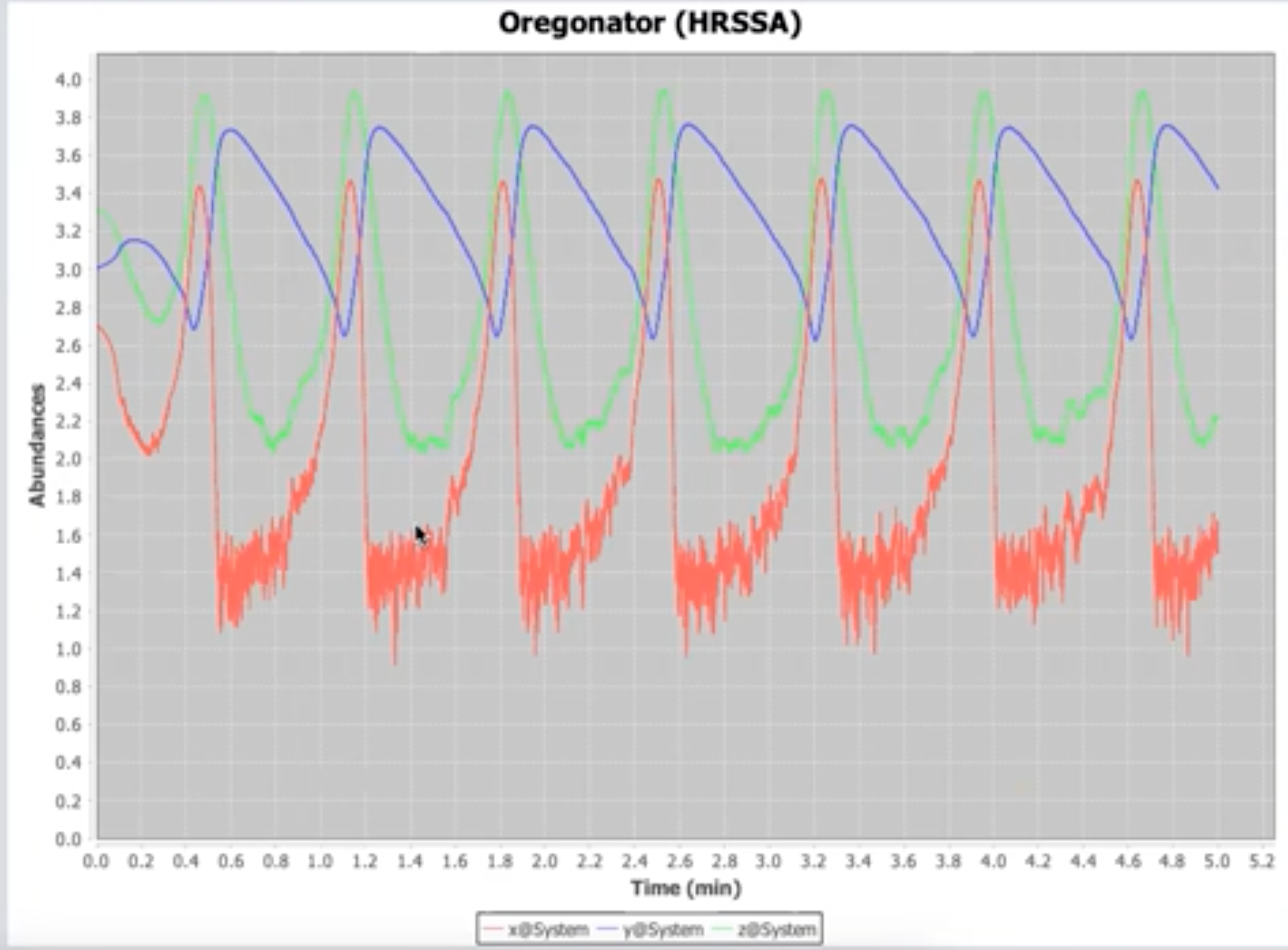
\includegraphics[width=0.6\textwidth]{HRSSA_oregonator.png}
  \caption{HSimulator HRSSA Oregonator}
  \label{fig:oregonator}
\end{figure}
\noindent
\textbf{Oregonator HRSSA:} (Figure \ref{fig:oregonator})  the algorithm applies the stochastic approach by starting from the deterministic setting.
In the advanced options we can insert additional specifications{]}.
If we apply steady state conditions (simulation length = 5, time sampling = 0.
0001), we observe a flat signal; the issue is that the stochastic simulation is applied to the subset of slow reactions.
If we change the parameters for deciding if something is fast or slow, we should see a change in the behaviour.
By working with smaller variables, we see something remarkable: noise is heavily present.
